\section{Introducci\'on}

En este trabajo pr\'actico vamos a desarrollar una implementaci\'on propia de traceroute. Traceroute es una consola de diagn\'ostico que permite seguir el recorrido de los paquetes, conocer cada nodo (router) por el que pasa, hasta llegar un host destino. Para poder conocer la ruta que recorren los paquetes e implementarlo, vamos a necesitar tener en cuenta las siguientes herramientas:

\begin{itemize}

\item Scapy: Herramiento usada en el trabajo pr\'actico anterior. Es una utilidad escrita en Python que nos servir\'a para crear y manipular paquetes, escanear, funciones de sniffer, entre otras.

\item ICMP (Internet Control Message Protocol): Es el sub protocolo de control y notificaci\'on de errores del Protocolo de Internet (IP). Se usa para enviar mensajes de error o de control, indicando por ejemplo que un servicio determinado no está disponible, o que un router o host no puede ser localizado, o que un paquete ha llegado al destino.
\begin{figure}[h]
	\begin{center}
    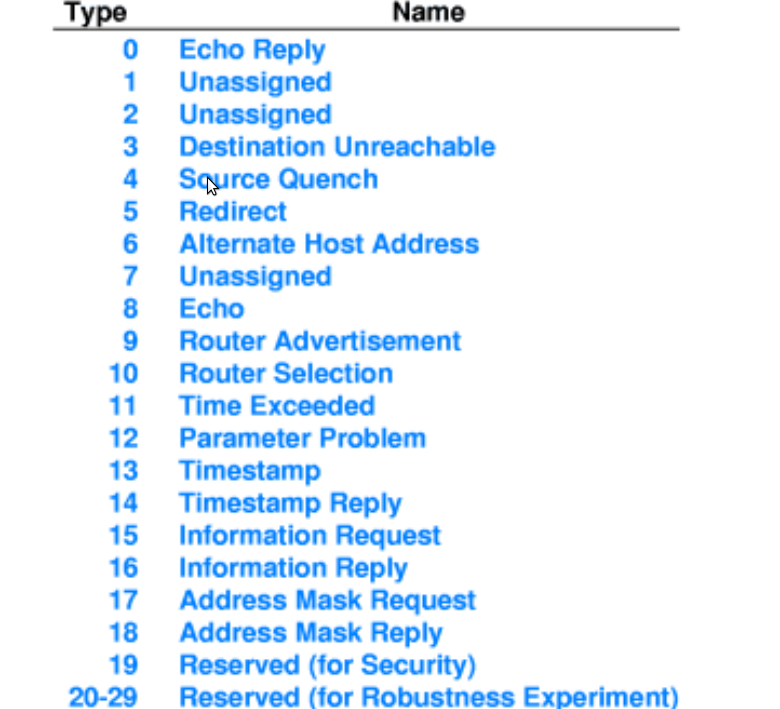
\includegraphics[width=0.5\textwidth]{ICMP_lista.png}
     \label{fig:ICMPlista} 
	\end{center}    
    \caption{Lista de algunos mensajes de control permitidos.}  
    
\end{figure}
\vspace{0.25cm}

\item TTL (time to live): No es mas que el tiempo de vida del paquete. Dentro del paquete enviado se setea dicho valor (entero) para saber cuando un paquete debe ser descartado, en caso que no llegue al destino. La forma en que funciona es, cada vez que el paquete pasa por un nodo, \'este \'ultimo le resta una unidad al valor que tenía cuando lo recibio, y lo propaga al siguiente nodo. En caso que el valor llegue a cero, el nodo descarta dicho paquete evitando que se siga propagando hasta su destino.

\item ICMP y TTL: Si a un paquete se le vence su TTL ($TTL = 0$), y \'este no est\'a en el nodo correspondiente a su host destino, nos llega un mensaje ICMP de "Time Exceeded" ($11$). En caso contrario, si un paquete llego a su host destino, sin importar el valor de su TTL, entonces via ICMP nos llegar\'a un mensaje de ''Echo Replay" ($0$).

\item RTT (Round-Trip delay Time): Es el tiempo que tarda un paquete de datos enviado desde un emisor en volver a este mismo, habiendo pasado por el receptor de destino. Es uno de los datos que nos muestra por pantalla las implementaciones hechas actualmente de traceroute. Con este valor podremos saber cuanto tardan los paquetes en llegar a cada nodo que intervienen en el recorrido hacia el host destino.

\end{itemize}

Una vez logrado el correcto funcionamiento del traceroute, con lo cual podremos conocer toda la ruta de un paquete, debemos tomar las estadísticas pertinentes para satisfacer los pedidos en las consignas dadas en el enunciado. Estos son:

\begin{itemize}

\item RTT promedio: Sobre un nodo tomamos su RTT promedio, esto nos sirve para estimar el tiempo veradero que tarda en llegar nuestro paquete hacia ese lugar, dado que en alguna instancia en particupal nos pudo haber dado un tiempo fuera de lo normal.

\item $\Delta$RTT: Es la diferencia entre el RTT promedio de un nodo con respecto a su antecesor.

\item Desv\'io Estandar para cada salto: Es la raiz cuadrada de la viaranza, la cual nos dice que tan dispersos son los datos tomados.

\item Test de hip\'otesis: Normal test\footnote{\url{https://en.wikipedia.org/wiki/Normal_distribution}} y Grubbs test\footnote{\url{https://en.wikipedia.org/wiki/Grubbs\%27_test_for_outliers}}. Adem\'as, para detectar outliers en el Grubbs test, necesitamos saber si el valor obtenido supera un rango que se deduce mediante t-student\footnote{\url{https://en.wikipedia.org/wiki/Student\%27s_t-distribution}}.

\end{itemize}

\subsection{Rutas Universitarias} 

Rutas a universidades por fuera de sudam\'erica: Como la idea que nos proponen, dado el test de Grubbs, es encontrar rutas submarinas (outliers), hemos optado por elegir universidades de distintos continentes en el cual hayan océanos de distancia con respecto a nuestra IP localizada en Argentina. Las elegidas son:

\begin{itemize}
\item Universidad 1
\item Universidad 2
\item Universidad 3
\end{itemize}